\documentclass[10pt, a4paper]{article}% size of txt = 10pt
\usepackage[top= 2cm,
			bottom = 2cm,
			left = 1.7cm,
			right = 1.7cm,
			footskip = 0.5cm,
			headsep = 0cm,
			headheight = 0cm
					]{geometry}
\usepackage{amsmath} % math packages
\usepackage{amsfonts}% math packages
\usepackage{amssymb} % math packages
\usepackage{graphicx} %package for including graphics
\usepackage{array}
\usepackage[thinlines]{easytable}
\usepackage{float}
\usepackage[section]{placeins}
\usepackage[hidelinks]{hyperref}
\usepackage[shortlabels]{enumitem}
\usepackage{svg}
\usepackage{bigstrut}
\usepackage{wrapfig,lipsum,booktabs}
\usepackage{subcaption}
\usepackage{xfrac}
\usepackage{pdfpages}
\usepackage{listings}
\usepackage{xcolor}


\usepackage{listings}
\usepackage{color} %red, green, blue, yellow, cyan, magenta, black, white
\definecolor{mygreen}{RGB}{28,172,0} % color values Red, Green, Blue
\definecolor{mylilas}{RGB}{170,55,241}

\definecolor{codegreen}{rgb}{0,0.6,0}
\definecolor{codegray}{rgb}{0.5,0.5,0.5}
\definecolor{codepurple}{rgb}{0.58,0,0.82}
\definecolor{backcolour}{rgb}{1,1,1}

\lstdefinestyle{mystyle}{
    backgroundcolor=\color{backcolour},   
    commentstyle=\color{codegreen},
    keywordstyle=\color{magenta},
    numberstyle=\tiny\color{codegray},
    stringstyle=\color{codepurple},
    basicstyle=\ttfamily\footnotesize,
    breakatwhitespace=false,         
    breaklines=true,                 
    captionpos=b,                    
    keepspaces=true,                 
    numbers=left,                    
    numbersep=5pt,                  
    showspaces=false,                
    showstringspaces=false,
    showtabs=false,                  
    tabsize=2
}
\lstset{style=mystyle}


%date format
\def\mydate{\leavevmode\hbox{\twodigits\day.\twodigits\month.\the\year}}
\def\twodigits#1{\ifnum#1<10 0\fi\the#1}

\usepackage{indentfirst}
\setlength{\parindent}{1cm}

\makeatletter
\newcommand{\thickhline}{%
    \noalign {\ifnum 0=`}\fi \hrule height 2pt
    \futurelet \reserved@a \@xhline
}
\newcolumntype{"}{@{\hskip\tabcolsep\vrule width 2pt\hskip\tabcolsep}}
\makeatother
\newcolumntype{?}{!{\vrule width 2pt}}
%%DOC ENVIROMENT%%%%%%%%%%%%%%%%%%%%%%%
\begin{document}
%Title 
\begin{flushleft}%% left justification
	\textbf{\Large{MKC-PKS: Úkol č. 3}}\hfill Filip Paul\\
	\large{Přenosová média, LAN, Ehternet \hfill\mydate}
\end{flushleft}
\section*{\large{\textbf{Uvažujte Ethernetový přepínač na rychlosti 1Gb/s, který pracuje na principu store-and-forward.
Určete jaké největší a nejmenší zpoždění vnese do komunikace mezi dvěma stanicemi 
oproti stavu, kdy by tyto stanice byly přímo propojeny kabelem. Zpoždění ve frontě a 
přepojovacím poli uvažujte nulové. (2b):}}}

\section*{\large{\textbf{Za jakých podmínek můžeme vytvořit síť Ethernet se vzdáleností stanic řádu 100km? (0,5b):}}}

\section*{\large{\textbf{Jak Ethernetový přepínač odliší značkovaný rámec podle 802.1q od rámce neznačkovaného? (0.5b)}}}

\section*{\large{\textbf{Předpokládejte, že oba přepínače mají na počátku prázdné tabulky MAC adres a podle 
následujícího popisu provozu tyto tabulky postupně sestavte. Ke všem níže uvedeným 
případům uveďte, jak který přepínač na daný rámec reaguje (kam ho přepošle). (2b)}}}

\begin{figure}[ht!]
	\centering
	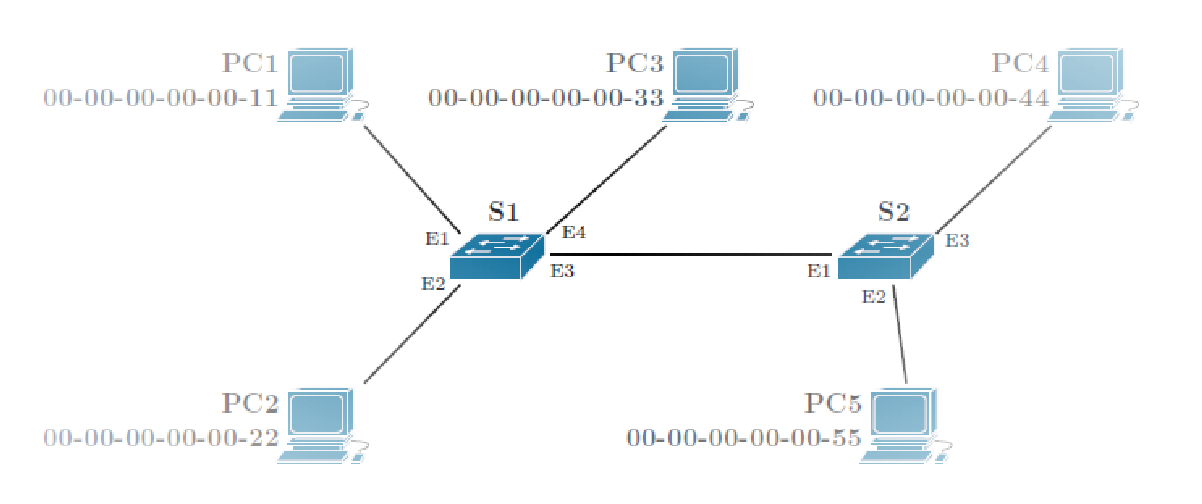
\includegraphics[width = 1\textwidth]{zadani_sit.eps}
	
\end{figure}
	

\end{document}